\chapter{FUNDAMENTAÇÃO TEÓRICA}
\label{chapter:fundamentacao}

Neste capítulo, são apresentados os fundamentos teóricos que sustentam a abordagem proposta, abrangendo conceitos de finanças e inteligência computacional. Inicialmente, são discutidos a teoria moderna do portfólio e o modelo Black-Litterman. Em seguida, são abordadas técnicas de aprendizado supervisionado, com ênfase no XGBoost, e conceitos de processamento de linguagem natural, análise de sentimento e modelos de linguagem aplicados a textos financeiros.

\section{Teoria Moderna do Portfólio}
\label{sec:teoria_portfolio}

A Teoria Moderna do Portfólio, proposta por Harry Markowitz, estabelece uma
abordagem quantitativa para a composição de carteiras de investimentos a
partir da relação entre retorno esperado e risco. O modelo de Média-Variância
considera que a escolha dos ativos deve levar em conta não apenas suas
características individuais, mas também a forma como seus retornos variam
conjuntamente. Dessa forma, a diversificação permite explorar as relações
de dependência entre os ativos na busca por diferentes combinações de risco
e retorno~\cite{markowitz}.

\subsection{Retorno e Risco de uma Carteira}
\label{subsec:retorno_risco}

O risco de um ativo é medido pela volatilidade dos seus retornos históricos, expressa matematicamente pelo desvio padrão. Já o retorno esperado representa a expectativa de ganho do investidor em um horizonte futuro~\cite{bodie_investments_vol1}. Segundo Markowitz, o retorno de uma carteira de investimentos pode ser obtido por meio da média ponderada dos retornos esperados dos ativos que a compõem, conforme a equação a seguir:

\begin{equation}
    R_p = \sum_{i=1}^{N} w_i \cdot R_i
\end{equation}

\noindent onde $R_p$ representa o retorno do portfólio, $w_i$ representa a proporção do capital alocada no $i$-ésimo ativo e $R_i$ o retorno esperado do $i$-ésimo ativo, em um universo de $N$ ativos.

O risco do portfólio $\sigma_p$ pode ser mensurado pela variância de seus retornos. Para tal, considerando $\mathbf{w}$ como o vetor de pesos e $\boldsymbol{\Sigma}$ como a matriz de covariâncias dos retornos dos ativos, a variância do portfólio é expressa por:

\begin{equation}
    \sigma_p^2 = \mathbf{w}^{T}\boldsymbol{\Sigma}\mathbf{w}.
    \label{eq:variancia_carteira}
\end{equation}

A Equação~(\ref{eq:variancia_carteira}) evidencia que o risco de uma carteira depende tanto da distribuição do capital entre os ativos quanto da covariância existente entre seus retornos. Desse modo, o risco agregado não corresponde à simples soma ponderada dos riscos individuais. Esta análise é fundamental para o princípio da diversificação, uma vez que ativos com diferentes padrões de variação podem interagir para mitigar o risco total da carteira.

\subsection{Diversificação e Fronteira Eficiente}
\label{subsec:diversificacao_fronteira}

A partir das estimativas de retorno esperado e da matriz de covariâncias, o problema de Média-Variância pode ser formulado como um modelo de otimização que busca equilibrar risco e retorno. Essa formulação pode assumir duas formas: minimizar a variância da carteira para um nível mínimo de retorno esperado ou maximizar o retorno esperado para um limite de risco. Na formulação apresentada a seguir, adota-se a primeira abordagem, buscando a carteira de menor risco que atenda ao retorno esperado estabelecido.

\begin{equation}
    \min_{\mathbf{w}} \quad \mathbf{w}^{T}\boldsymbol{\Sigma}\mathbf{w},
    \label{eq:markowitz_objetivo}
\end{equation}

sujeito às seguintes restrições:

\begin{equation}
    \mathbf{w}^{T}\boldsymbol{\mu} = R^{*},
    \label{eq:markowitz_retorno}
\end{equation}

e

\begin{equation}
    \mathbf{1}^{T}\mathbf{w} = 1.
    \label{eq:markowitz_soma_pesos}
\end{equation}

\noindent onde $\boldsymbol{\mu}$ é o vetor de retornos esperados dos ativos individuais, $R^*$ representa o retorno esperado exigido para a carteira e $\mathbf{1}$ é um vetor de uns. A restrição apresentada na Equação~\eqref{eq:markowitz_soma_pesos} garante que a soma dos pesos dos ativos seja igual a $1$, ou seja, que $100\%$ do capital disponível seja alocado.
\vspace{0.5cm}

A solução desse problema de otimização para diferentes níveis de retorno esperado produz um conjunto de carteiras ótimas, o qual estabelece a relação de compromisso entre risco e retorno. Esse conjunto delimita a chamada fronteira eficiente, composta pelas carteiras que apresentam o menor risco possível para cada nível de retorno exigido~\cite{markowitz}.

\begin{figure}[H]
    \centering
    \caption{Fronteira eficiente de ativos de risco}
    \label{fig:fronteira_bodie}
    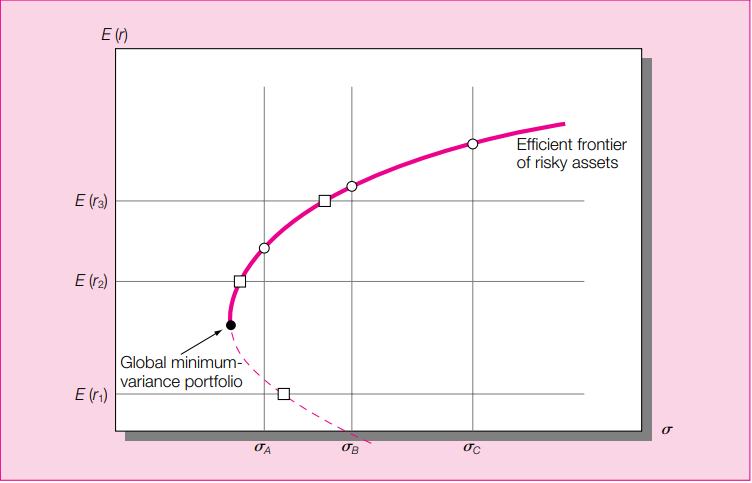
\includegraphics[width=0.8\textwidth]{02_Fundamentacao/figures/fronteira eficiente.png}
    
    Fonte: \cite{bodie_investments_vol1}
\end{figure}

\section{Modelo de Black-Litterman}
\label{sec:black_litterman}

O modelo BL foi desenvolvido por Fischer Black e Robert Litterman como uma
abordagem para a estimação de retornos esperados que combina informações
provenientes do equilíbrio de mercado com visões específicas sobre os
ativos. A estrutura permite incorporar diferentes níveis de incerteza
associados às informações utilizadas no processo de estimação
~\cite{blacklitterman}.

\subsection{Equilíbrio de Mercado e Otimização Reversa}
\label{subsec:equilibrio_mercado}

No modelo de BL, os retornos de equilíbrio são obtidos a partir da composição observada do mercado. Em vez de definir diretamente os retornos esperados, realiza-se o procedimento inverso: parte-se dos pesos de mercado e da matriz de covariâncias para determinar quais retornos seriam compatíveis com essa alocação~\cite{helitterman1999}.

Esse procedimento é denominado otimização reversa. Considerando $\boldsymbol{\Sigma}$ como a matriz de covariâncias dos retornos e $\mathbf{w}_{\mathrm{mkt}}$ como o vetor de pesos dos ativos no portfólio de mercado, em que cada peso representa a proporção da capitalização do ativo em relação ao mercado total, o vetor de retornos de equilíbrio, $\boldsymbol{\pi}$, é expresso por:

\begin{equation}
    \boldsymbol{\pi} = \delta\boldsymbol{\Sigma}\mathbf{w}_{\mathrm{mkt}},
    \label{eq:bl_prior}
\end{equation}

\noindent em que $\delta$ representa o coeficiente de aversão ao risco do mercado, que pode ser estimado pela razão entre o retorno esperado do mercado acima da taxa livre de risco e a variância de seus retornos. Esse coeficiente expressa a compensação em retorno exigida pelos investidores por unidade de risco assumida.~\cite{sharpe1964}.



O vetor $\boldsymbol{\pi}$ constitui a estimativa de retorno de equilíbrio utilizada como ponto de partida no modelo. Dessa forma, o BL extrai as informações presentes na própria capitalização de mercado antes da incorporação das expectativas subjetivas do investidor.

\subsection{Incorporação de Visões}
\label{subsec:bl_views}

Além dos retornos de equilíbrio, o modelo permite incorporar as expectativas subjetivas do investidor sobre os retornos esperados dos ativos. Essas visões podem ser absolutas ou relativas, sendo estruturadas matematicamente por meio de uma matriz $\mathbf{P}$ e de um vetor $\mathbf{Q}$~\cite{idzorek2005}.

A matriz $\mathbf{P}$ identifica os ativos envolvidos em cada visão, enquanto o vetor $\mathbf{Q}$ contém os valores de retorno associados a elas. Considerando a incerteza inerente a essas projeções, adiciona-se um termo de erro, de modo que a formulação é expressa por:

\begin{equation}
    \mathbf{P}\boldsymbol{\mu} = \mathbf{Q} + \boldsymbol{\varepsilon}, \qquad \boldsymbol{\varepsilon} \sim \mathcal{N}(\mathbf{0},\boldsymbol{\Omega}),
    \label{eq:bl_views}
\end{equation}

\noindent em que $\boldsymbol{\mu}$ é o vetor de retornos esperados dos ativos e $\boldsymbol{\varepsilon}$ é o vetor de erros, com distribuição normal de média nula e matriz de covariâncias $\boldsymbol{\Omega}$. Uma forma de estimar essa matriz consiste em calcular as diferenças entre os retornos observados e os previstos por cada visão e, em seguida, obter as covariâncias amostrais desses erros. Dessa forma, visões com erros mais dispersos recebem maior incerteza.

Uma visão absoluta especifica o retorno esperado de um ativo,
independentemente do desempenho dos demais. Por exemplo, esperar
que o ativo A apresente retorno de $5\%$ em determinado período
corresponde à relação $\mu_A = 0{,}05$. Nesse caso, a linha
correspondente da matriz $\mathbf{P}$ recebe o valor $1$ na posição
do ativo A e zero nas demais, enquanto o elemento de $\mathbf{Q}$
recebe $0{,}05$.

Uma visão relativa estabelece uma diferença esperada entre os
retornos de dois ativos ou grupos de ativos. Por exemplo, esperar
que o ativo A supere o ativo B em dois pontos percentuais no mesmo
período corresponde à relação $\mu_A - \mu_B = 0{,}02$. Nesse caso,
a linha de $\mathbf{P}$ recebe $1$ na posição de A, $-1$ na posição
de B e zero nas demais, enquanto o elemento de $\mathbf{Q}$
recebe $0{,}02$. Essas relações representam expectativas sujeitas
à incerteza, que o modelo combina com os retornos de equilíbrio.

A influência dessas visões na estimativa final depende da incerteza
representada pela matriz $\boldsymbol{\Omega}$. Quanto maior a
variância associada a uma visão, menor a confiança atribuída a ela
e, consequentemente, menor sua influência na atualização dos
retornos de equilíbrio. A estimativa resultante dessa combinação
é denominada retorno posterior.

\subsection{Retorno Posterior e Incerteza das Visões}
\label{subsec:bl_posterior}

A combinação entre o retorno de equilíbrio e as visões do investidor resulta em uma nova estimativa para os retornos esperados. Considerando $\tau$ como um escalar que reflete o nível de incerteza associado à estimativa do retorno de equilíbrio, o retorno posterior é dado por:

\begin{equation}
    \boldsymbol{\mu}_{BL} = \left[ (\tau\boldsymbol{\Sigma})^{-1} + \mathbf{P}^{T}\boldsymbol{\Omega}^{-1}\mathbf{P} \right]^{-1} \left[ (\tau\boldsymbol{\Sigma})^{-1}\boldsymbol{\pi} + \mathbf{P}^{T}\boldsymbol{\Omega}^{-1}\mathbf{Q} \right].
    \label{eq:bl_posterior}
\end{equation}

\noindent onde $\tau$ é uma constante de escala que pondera a incerteza da distribuição de partida, e os demais termos seguem as definições anteriores.

A Equação~\eqref{eq:bl_posterior} funciona fundamentalmente como uma média ponderada das duas fontes de informação: a estimativa de equilíbrio ($\boldsymbol{\pi}$) e o vetor de visões ($\mathbf{Q}$). A ponderação de cada componente é inversamente proporcional às suas respectivas matrizes de incerteza, de modo que a fonte de informação com menor variância exerce maior peso na determinação final~\cite{meucci2005}.

Dessa forma, o modelo Black-Litterman oferece uma estrutura matematicamente consistente para combinar o equilíbrio de mercado com as projeções do analista, ajustando o impacto dessas projeções de acordo com o grau de confiança atribuído a cada uma. O vetor resultante, $\boldsymbol{\mu}_{BL}$, substitui as estimativas históricas tradicionais e passa a ser utilizado como o vetor de retornos esperados no problema de otimização da carteira.

\begin{figure}[htb]
    \centering
    \caption{\label{fig:black_litterman_flow}Fluxograma da combinação de retornos no modelo Black-Litterman}
    \resizebox{\textwidth}{!}{%
    \begin{tikzpicture}[
        node distance=0.8cm and 0.4cm,
        box/.style={draw, rectangle, align=center, minimum height=0.8cm, inner sep=5pt, font=\small},
        bigbox/.style={draw, rectangle, align=center, inner sep=6pt, font=\small},
        arrow/.style={->, >=stealth, thick}
    ]
        % Prior Side (Left)
        \node[box] (lambda) {Coeficiente de Aversão ao Risco\\ $\lambda = \frac{E(r) - r_f}{\sigma^2}$};
        \node[box, right=of lambda] (sigma) {Matriz de Covariância\\ $(\boldsymbol{\Sigma})$};
        \node[box, right=of sigma] (wmkt) {Pesos de Cap. de Mercado\\ $(\mathbf{w}_{mkt})$};

        \node[bigbox, below=0.6cm of sigma, text width=7.5cm] (implied) {
            Vetor de Retorno de Equilíbrio Implícito\\ $\boldsymbol{\Pi} = \lambda \boldsymbol{\Sigma} \mathbf{w}_{mkt}$
        };

        \node[bigbox, below=0.6cm of implied, text width=6cm] (prior) {
            Distribuição de Equilíbrio\\
            \vspace{0.1cm}
            $N \sim (\boldsymbol{\Pi}, \tau\boldsymbol{\Sigma})$
        };

        % Views Side (Right)
        \node[box, right=1.2cm of wmkt] (views) {Visões do Investidor\\ ($Q$)};
        \node[box, right=of views] (omega) {Incerteza das Visões\\ ($\Omega$)};

        \node[bigbox, below=1.8cm of views, xshift=0.8cm, text width=5.5cm] (view_dist) {
            Distribuição das Visões\\
            \vspace{0.1cm}
            $N \sim (Q, \Omega)$
        };

        % Combined (Bottom)
        \node[bigbox, below=1.0cm of prior, xshift=2.0cm, text width=11cm] (posterior) {
            Nova Distribuição Combinada de Retornos\\
            \vspace{0.2cm}
            $N \sim \left( E[R], \left[ (\tau\boldsymbol{\Sigma})^{-1} + P^T \Omega^{-1} P \right]^{-1} \right)$
        };

        % Arrows
        \draw[arrow] (lambda) -- (implied);
        \draw[arrow] (sigma) -- (implied);
        \draw[arrow] (wmkt) -- (implied);
        \draw[arrow] (implied) -- (prior);

        \draw[arrow] (views) -- (view_dist);
        \draw[arrow] (omega) -- (view_dist);

        \draw[arrow] (prior) -- (posterior);
        \draw[arrow] (view_dist) -- (posterior);

    \end{tikzpicture}%
    }
    Fonte: Adaptado de \cite{walters2014black}
\end{figure}

\section{Aprendizado Supervisionado}
\label{subsec:aprendizado_supervisionado}

O aprendizado supervisionado é uma técnica de aprendizado de máquina que utiliza um conjunto de observações em que as variáveis de entrada estão associadas a valores conhecidos de uma variável alvo~\cite{hastie2009}. Por meio do treinamento, é possível identificar padrões e relações inerentes a esses dados. Considere um conjunto formado por pares $(\mathbf{x}_i,y_i)$, em que $\mathbf{x}_i$ representa o vetor de variáveis independentes e $y_i$ representa a variável alvo. O objetivo consiste em estimar uma função:

\begin{equation}
    \hat{y}=f(\mathbf{x}),
    \label{eq:supervised_learning}
\end{equation}

\noindent capaz de produzir estimativas da variável alvo a partir de novas observações, o que reflete a capacidade de generalização do modelo.

Os problemas de aprendizado supervisionado podem ser divididos, entre outras abordagens, em tarefas de regressão e de classificação. Na regressão, a variável alvo assume valores contínuos, enquanto na classificação, ela mapeia os dados em categorias discretas.

Neste trabalho, essas duas formas de aprendizado são utilizadas de maneira complementar. A regressão é empregada para estimar a magnitude dos retornos futuros dos ativos, enquanto a classificação é utilizada para determinar sua direção esperada (movimento de alta ou baixa).

\subsection{Árvores de Decisão e Boosting}
\label{subsec:arvores_boosting}

As árvores de decisão representam uma estrutura hierárquica de
regras condicionais aplicadas às variáveis de entrada. Durante o
treinamento, cada nó interno divide as observações em grupos,
buscando reduzir a impureza ou o erro de previsão.

Essa estrutura é composta por um nó raiz, que reúne inicialmente
todas as observações, nós internos, que realizam os testes, e nós
folha, que fornecem as previsões. Cada teste verifica uma condição
sobre uma variável de entrada. Por exemplo, pode-se verificar se
o retorno de um ativo no período anterior foi maior que $1\%$,
separando as observações em dois grupos conforme a resposta.
Esse processo se repete até que a observação alcance uma folha.
Em problemas de regressão, a previsão dessa folha geralmente
corresponde à média dos valores da variável que se deseja prever
nas observações de treinamento agrupadas nela.

Uma única árvore, no entanto, pode apresentar elevada variância
e suscetibilidade a ruídos, especialmente quando cresce sem
restrições. Métodos de \textit{ensemble} buscam melhorar a
capacidade de generalização por meio da combinação de múltiplos
modelos preditivos. Um exemplo é o \textit{boosting}, no qual os
modelos são construídos sequencialmente, de modo que cada novo
modelo procure corrigir os erros da combinação dos anteriores.
No caso do \textit{gradient boosting}, essa correção é orientada
pelo gradiente da função de perda.

No \textit{Gradient Boosting}, a previsão final resulta da soma
das contribuições ponderadas das árvores de regressão,
acrescida de uma previsão inicial~\cite{friedman2001}:

\begin{equation}
    \hat{y}_i = F_0(\mathbf{x}_i)
    + \eta \sum_{k=1}^{K} \rho_k f_k(\mathbf{x}_i),
    \label{eq:gradient_boosting}
\end{equation}

\noindent em que $\hat{y}_i$ é a previsão para a observação $i$,
$\mathbf{x}_i$ é seu vetor de entrada e $F_0(\mathbf{x}_i)$
é a previsão inicial. Cada função $f_k$ representa uma árvore
de regressão que busca corrigir os erros das etapas anteriores,
e $K$ é o número de árvores. O coeficiente $\rho_k$ pondera
a contribuição da árvore $k$ e é escolhido para reduzir o erro
do modelo, enquanto $\eta$ é a taxa de aprendizado, que controla
a intensidade das atualizações.

Essa arquitetura aditiva combina árvores de regressão para
melhorar progressivamente as previsões do modelo. A cada etapa,
uma nova árvore é ajustada para reduzir os erros da combinação
anterior, segundo a função de perda adotada. Dessa forma, o
modelo é refinado por meio de correções sucessivas.

\begin{figure}[H]
    \centering
    \caption{Arquitetura do modelo de \textit{Gradient Boosting}.}
    \label{fig:diagrama_boosting}
    \resizebox{0.85\linewidth}{!}{%
    \begin{tikzpicture}[
        >=Stealth,
        % Estilos dos nós
        databox/.style={draw, dashed, thick, minimum width=2.2cm, minimum height=1.2cm, align=center, fill=gray!5},
        treeleaf/.style={circle, fill=black, inner sep=0pt, minimum size=5pt},
        treeroot/.style={circle, fill=black, inner sep=0pt, minimum size=7pt},
        textnode/.style={align=center, font=\footnotesize},
        arrowtext/.style={above, sloped, font=\scriptsize}
    ]

    % Macro para desenhar as pequenas árvores de decisão
    \def\drawtree#1#2{
        % #1 é o prefixo do nó, #2 é a coordenada central
        \node[treeroot] (#1_root) at (#2) {};
        \node[treeleaf] (#1_L) at ($(#2) + (-0.6,-0.7)$) {};
        \node[treeleaf] (#1_R) at ($(#2) + (0.6,-0.7)$) {};
        \node[treeleaf] (#1_LL) at ($(#2) + (-0.9,-1.4)$) {};
        \node[treeleaf] (#1_LR) at ($(#2) + (-0.3,-1.4)$) {};
        \node[treeleaf] (#1_RL) at ($(#2) + (0.3,-1.4)$) {};
        \node[treeleaf] (#1_RR) at ($(#2) + (0.9,-1.4)$) {};
        
        \draw[->, thick] (#1_root) -- (#1_L);
        \draw[->, thick] (#1_root) -- (#1_R);
        \draw[->, thick] (#1_L) -- (#1_LL);
        \draw[->, thick] (#1_L) -- (#1_LR);
        \draw[->, thick] (#1_R) -- (#1_RL);
        \draw[->, thick] (#1_R) -- (#1_RR);
    }

    % 1. Desenhar as caixas de Dados
    \node[databox] (D1) at (0, 3.5) {Dados};
    \node[databox] (D2) at (3.5, 3.5) {Dados\\Ponderados};
    \node[databox] (D3) at (7.0, 3.5) {Dados\\Ponderados};
    \node[databox] (DX) at (11.0, 3.5) {Dados\\Ponderados};

    % 2. Desenhar as Árvores
    \drawtree{T1}{0,0}
    \drawtree{T2}{3.5,0}
    \drawtree{T3}{7.0,0}
    \drawtree{TX}{11.0,0}

    % Reticências entre a árvore 3 e a árvore X
    \node at (9.0, 1.5) {\Huge $\dots$};

    % Legendas das árvores
    \node[textnode, below=1.6cm of T1_root] (T1_label) {Árvore 1\\(Classificador fraco)};
    \node[textnode, below=1.6cm of T2_root] (T2_label) {Árvore 2\\(Classificador fraco)};
    \node[textnode, below=1.6cm of T3_root] (T3_label) {Árvore 3\\(Classificador fraco)};
    \node[textnode, below=1.6cm of TX_root] (TX_label) {Árvore X\\(Classificador fraco)};

    % 3. Desenhar o nó do Ensemble
    \node[treeroot, minimum size=10pt] (E_center) at (5.5, -4.5) {};
    \foreach \a in {18, 90, 162, 234, 306} {
        \node[treeleaf] (E_arm\a) at ($(E_center) + (\a:0.5)$) {};
        \draw[thick] (E_center) -- (E_arm\a);
    }
    \node[textnode, below=0.7cm of E_center] (E_label) {\textbf{Predição do \textit{Ensemble}}\\(Classificador forte)};

    % 4. Desenhar as Setas
    % Setas de Ajuste
    \draw[->, thick] (D1) -- node[left, font=\scriptsize] {Ajuste} (T1_root);
    \draw[->, thick] (D2) -- node[left, font=\scriptsize] {Ajuste} (T2_root);
    \draw[->, thick] (D3) -- node[left, font=\scriptsize] {Ajuste} (T3_root);
    \draw[->, thick] (DX) -- node[left, font=\scriptsize] {Ajuste} (TX_root);

    % Setas de Resíduos
    \draw[->, thick] (T1_root) -- node[arrowtext] {Resíduos da Predição} (D2);
    \draw[->, thick] (T2_root) -- node[arrowtext] {Resíduos da Predição} (D3);
    \draw[->, thick] (T3_root) -- node[arrowtext] {Resíduos da Predição} (9.0, 2.5);

    % Setas de Predição Final
    \draw[->, dashed, thick] (T1_label.south) -- node[arrowtext] {Predição} (E_center);
    \draw[->, dashed, thick] (T2_label.south) -- node[arrowtext] {Predição} (E_center);
    \draw[->, dashed, thick] (T3_label.south) -- node[arrowtext] {Predição} (E_center);
    \draw[->, dashed, thick] (TX_label.south) -- node[arrowtext] {Predição} (E_center);

    \end{tikzpicture}%
    }\\
    Adaptado de \cite{deng2021ensemble}.
\end{figure}

\subsection{XGBoost}
\label{subsec:xgboost}

O XGBoost é uma implementação otimizada do algoritmo de \textit{Gradient Boosting} baseada em árvores de decisão, que se destaca pelo rigor matemático na minimização da função objetivo e pela eficiência computacional~\cite{chen2016xgboost}.

Para a $t$-ésima árvore adicionada ao modelo, a função objetivo a ser minimizada é dada por:

\begin{equation}
    \mathcal{L}^{(t)} = \sum_{i=1}^{n} l\left(y_i, \hat{y}_i^{(t-1)} + f_t(\mathbf{x}_i)\right) + \Omega(f_t),
    \label{eq:xgboost_objective}
\end{equation}

\noindent em que $l$ é uma função de perda diferenciável que mensura a divergência entre a meta $y_i$ e a previsão anterior $\hat{y}_i^{(t-1)}$, e $\Omega(f_t)$ é o termo de regularização que penaliza a complexidade da nova árvore $f_t$, definido por:

\begin{equation}
    \Omega(f_t) = \gamma T + \frac{1}{2}\lambda \sum_{j=1}^{T} w_j^2,
    \label{eq:xgboost_reg}
\end{equation}

\noindent sendo $T$ o número de folhas da árvore, $w_j$ o peso do $j$-ésimo nó folha, $\gamma$ a penalidade por adição de folhas e $\lambda$ o parâmetro de regularização $L_2$ sobre os pesos.

Para otimizar a Equação~\eqref{eq:xgboost_objective} de forma rápida, o algoritmo emprega uma expansão em série de Taylor de segunda ordem na função de perda:

\begin{equation}
    \mathcal{L}^{(t)} \approx \sum_{i=1}^{n} \left[ l\left(y_i, \hat{y}_i^{(t-1)}\right) + g_i f_t(\mathbf{x}_i) + \frac{1}{2} h_i f_t^2(\mathbf{x}_i) \right] + \Omega(f_t),
    \label{eq:taylor_expansion}
\end{equation}

\noindent em que $g_i$ e $h_i$ representam, respectivamente,
as derivadas de primeira e segunda ordem da função de perda
em relação à previsão, avaliadas na etapa anterior:
\begin{equation}
    g_i =
    \left.
    \frac{\partial l(y_i,\hat{y}_i)}{\partial \hat{y}_i}
    \right|_{\hat{y}_i=\hat{y}_i^{(t-1)}},
    \qquad
    h_i =
    \left.
    \frac{\partial^2 l(y_i,\hat{y}_i)}{\partial \hat{y}_i^2}
    \right|_{\hat{y}_i=\hat{y}_i^{(t-1)}}.
\end{equation}

Removendo os termos constantes no passo $t$, a função objetivo simplificada torna-se:

\begin{equation}
    \tilde{\mathcal{L}}^{(t)} = \sum_{i=1}^{n} \left[ g_i f_t(\mathbf{x}_i) + \frac{1}{2} h_i f_t^2(\mathbf{x}_i) \right] + \gamma T + \frac{1}{2}\lambda \sum_{j=1}^{T} w_j^2.
\end{equation}

Em aplicações financeiras, modelos baseados em árvores e
\textit{boosting} podem ser utilizados na previsão de retornos,
na seleção de ações e na construção de carteiras. Por exemplo,
informações sobre retornos passados, liquidez e volatilidade
podem ser combinadas para estimar o desempenho futuro dos ativos
e apoiar sua ordenação conforme o retorno previsto.
Em~\cite{gu2020} investigam-se métodos de aprendizado
de máquina, incluindo árvores com \textit{boosting}, na previsão
de retornos de ações, destacando a importância dessas variáveis
e das relações não lineares entre elas. No presente trabalho,
o XGBoost é utilizado para gerar previsões de retorno que
contribuem para a construção das visões do modelo Black-Litterman.

\section{Processamento de Linguagem Natural e Análise de Sentimento}
\label{sec:nlp_sentimento}

O Processamento de Linguagem Natural (PLN) é uma área dedicada à modelagem computacional da linguagem humana. No domínio textual, busca-se representar a organização e o significado dos textos para extrair informações e realizar tarefas como identificar entidades, reconhecer relações e classificar documentos. O desafio consiste na associação de expressões linguísticas às informações relevantes para cada tarefa, por exemplo, a presença de uma palavra, isoladamente, pode ser insuficiente para determinar o sentido de uma afirmação. Como se pode observar na frase ``o serviço não foi satisfatório'' onde o contexto altera a avaliação que seria atríbuida ao termo ``satisfatório''~\cite{goldberg2016primer}.

\subsection{Fundamentos de NLP}
\label{subsec:fundamentos_nlp}

Entre as abordagens clássicas de análise textual, a mineração de textos (\textit{text mining}) procura identificar padrões e extrair informações de coleções de documentos. Uma estratégia recorrente consiste em representar cada documento por um vetor de contagens de palavras, conhecido como \textit{bag-of-words}, ou por pesos TF-IDF (\textit{term frequency--inverse document frequency}), que combinam a frequência de um termo no documento com sua frequência na coleção. Essas representações podem alimentar algoritmos de classificação e agrupamento. Entretanto, ao desconsiderarem a ordem das palavras, limitam a representação de relações como a negação e a dependência entre termos~\cite{manning2008ir}.

O aprendizado profundo (\textit{deep learning}) permite aprender representações vetoriais e relações entre elementos do texto durante o treinamento. As redes neurais recorrentes (\textit{Recurrent Neural Networks} -- RNNs) processam sequências mantendo um estado interno atualizado a cada elemento, de modo que a representação de uma palavra pode incorporar informações das posições anteriores. Variantes como as redes LSTM (\textit{Long Short-Term Memory}) introduzem mecanismos de controle da memória para facilitar o aprendizado de dependências ao longo da sequência~\cite{goldberg2016primer}.

A ~\ref{fig:rnn_caracteres} ilustra uma RNN que utiliza
a entrada atual e o estado anterior para prever o próximo
caractere da palavra ``modelos''.

\begin{figure}[htbp]
    \centering
    \caption{Rede neural recorrente aplicada à previsão
    do próximo caractere de uma palavra.}
    \label{fig:rnn_caracteres}
    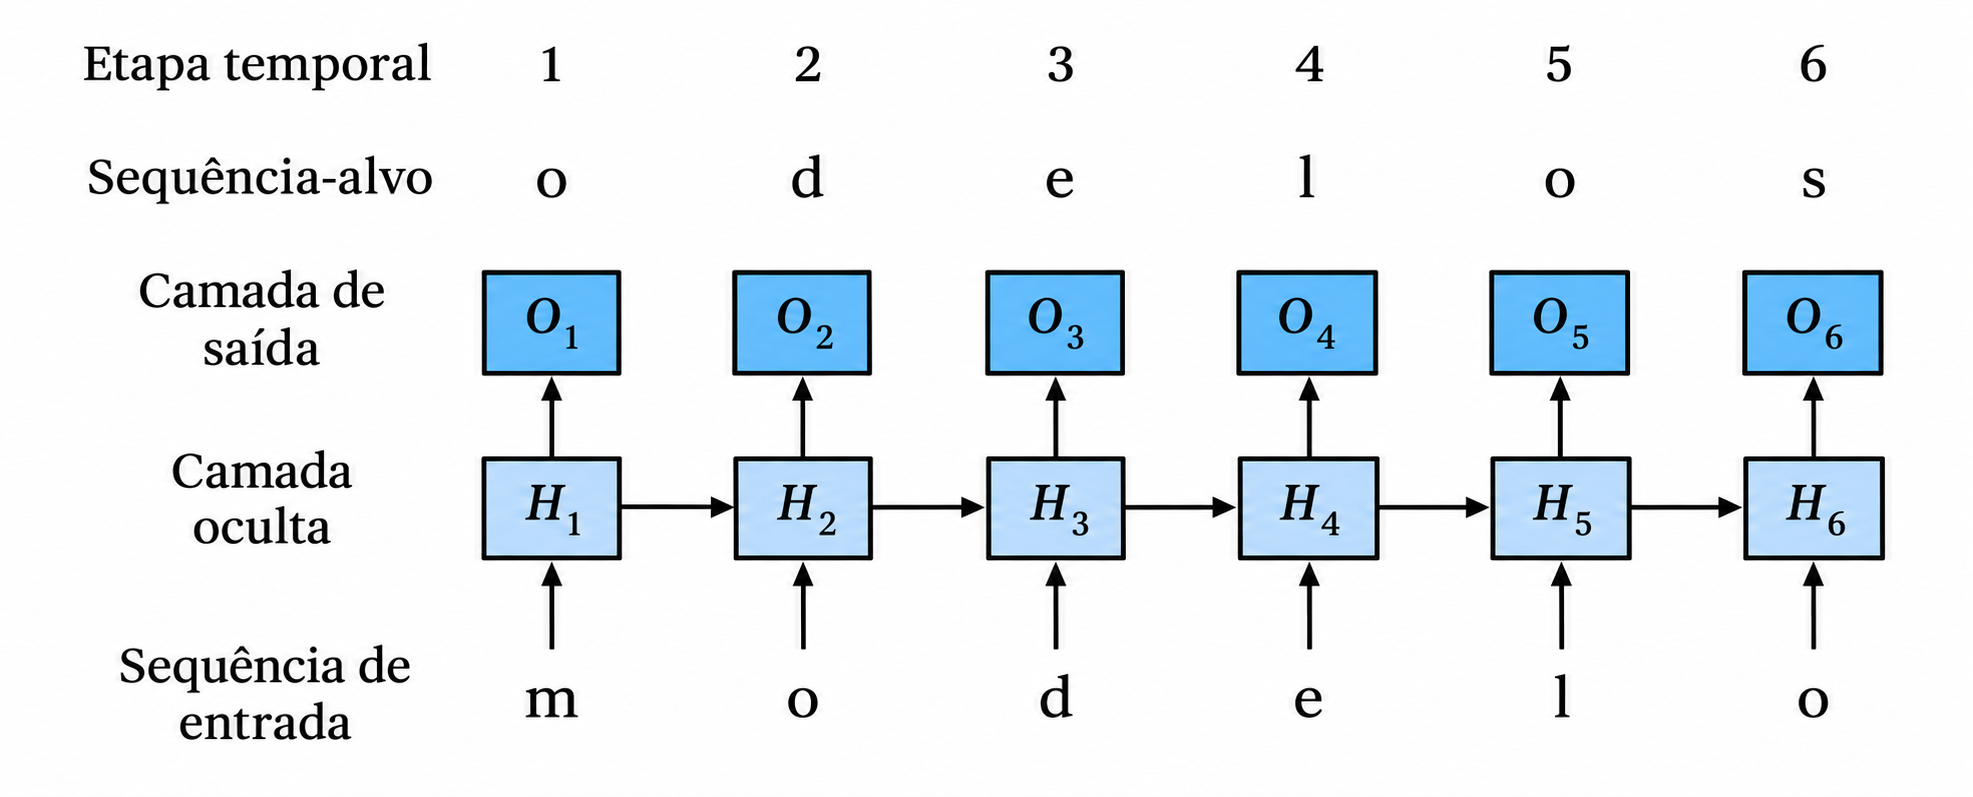
\includegraphics[width=0.7\textwidth]
    {02_Fundamentacao/figures/adaptado rnn.png}

    \par\smallskip
    Fonte: Adaptado de \cite{zhang2023dive}.
\end{figure}

\newpage

A arquitetura Transformer utiliza mecanismos de atenção para relacionar diferentes posições de uma sequência, dispensando a recorrência. Na autoatenção, a representação de cada elemento é calculada a partir de uma combinação ponderada das representações dos elementos aos quais ele pode atender. Isso permite incorporar informações de outras partes do texto conforme as relações aprendidas pelo modelo~\cite{vaswani2017}. A ~\ref{fig:exemplo_autoatencao} ilustra esses pesos de atenção.

\begin{figure}[htbp]
    \centering
    \caption{Visualização dos pesos do mecanismo de autoatenção.}
    \label{fig:exemplo_autoatencao}
    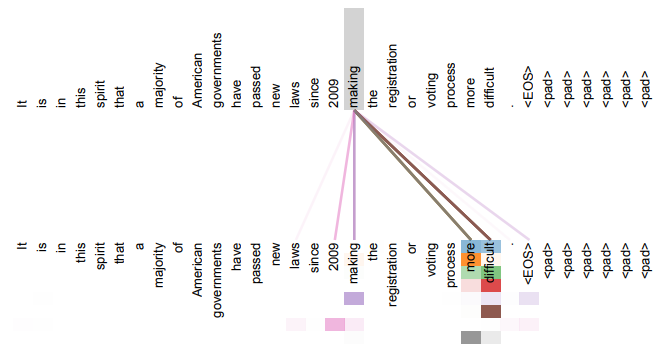
\includegraphics[width=0.8\textwidth]{02_Fundamentacao/figures/self attention.png} 
\par\smallskip Fonte: \cite{vaswani2017}
\end{figure}

Entre os modelos baseados nessa arquitetura, o BERT
(\textit{Bidirectional Encoder Representations from Transformers})
utiliza o contexto à esquerda e à direita para aprender
representações dos elementos de entrada. Seu pré-treinamento
inclui a recuperação de partes do texto ocultadas durante o
treinamento, e o modelo pode ser ajustado para tarefas específicas,
como a classificação de textos~\cite{devlin2019bert}.
A ~\ref{fig:bert} apresenta as diferenças entre os
esquemas de contextualização do BERT, do GPT original e do ELMo.

\begin{figure}[htbp]
    \centering
    \caption{Esquemas de contextualização do BERT, do GPT original e do ELMo.}
    \label{fig:bert}
    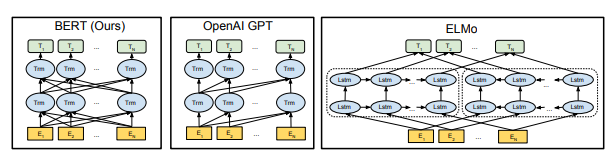
\includegraphics[width=0.8\textwidth]{02_Fundamentacao/figures/bert.png} 
\par\smallskip Fonte: \cite{devlin2019bert}
\end{figure}

\subsection{Modelos de Linguagem de Grande Escala}
\label{subsec:llms}

Os modelos de linguagem de grande escala (\textit{Large Language
Models} -- LLMs) aprendem padrões linguísticos a partir de grandes
volumes de dados. Seu desenvolvimento está associado ao uso da
arquitetura Transformer, cujos mecanismos de atenção permitem
modelar relações entre os elementos de uma sequência
textual~\cite{vaswani2017}.

Entre esses modelos, os LLMs generativos autorregressivos, como
os da família GPT, produzem texto progressivamente a partir do
conteúdo anterior. Embora seu mecanismo de resposta seja
generativo, eles também podem realizar tarefas discriminativas,
como a classificação. Nesse caso, são fornecidos o texto a ser
analisado, as instruções e as categorias permitidas, e o modelo
gera uma resposta correspondente a um dos rótulos. Essa utilização
pode ocorrer em regime \textit{zero-shot}, sem exemplos da tarefa
no contexto fornecido, ou \textit{few-shot}, com alguns exemplos
de entradas e saídas, sem atualização dos parâmetros durante
a aplicação~\cite{brown2020language}.

As instruções fornecidas ao modelo, denominadas \textit{prompt},
estabelecem o critério de classificação e o formato esperado da
resposta. Por isso, a definição das categorias e a clareza das
instruções são aspectos relevantes para a aplicação.

Neste trabalho, utiliza-se um LLM generativo em regime
\textit{zero-shot} para atribuir categorias de sentimento a textos,
sem treinamento supervisionado adicional com os documentos da
amostra. A caracterização dessa tarefa é apresentada a seguir.

\subsection{Análise de Sentimento}
\label{subsec:analise_sentimento}

A análise de sentimento busca identificar e caracterizar avaliações, opiniões e orientações expressas em textos. Uma de suas formulações é a classificação de polaridade, na qual o conteúdo é associado a categorias como positivo, negativo e neutro em relação a um objeto de interesse. A tarefa pode ser realizada no nível de um documento, de uma sentença ou de um aspecto específico de uma entidade. Um mesmo texto pode, por exemplo, avaliar favoravelmente a qualidade de um produto e desfavoravelmente seu preço, exigindo a identificação do alvo de cada avaliação~\cite{pang2008opinion}.

A polaridade depende da composição da mensagem. Expressões de negação, intensidade e contraste podem alterar a interpretação de termos que, isoladamente, sugeririam uma avaliação distinta. Além disso, a ausência de opinião explícita não elimina a possibilidade de uma informação ter implicações favoráveis ou desfavoráveis para o objeto analisado. Por isso, a definição das categorias deve esclarecer o que se pretende avaliar e qual é o alvo da classificação~\cite{du2024financial}.

As estratégias para realizar essa tarefa incluem métodos baseados em léxicos, que associam palavras a orientações previamente estabelecidas, e métodos supervisionados, que aprendem a classificar a partir de exemplos rotulados. Modelos de linguagem pré-treinados podem ser ajustados com esses exemplos, enquanto LLMs generativos permitem formular a classificação por instruções. Essas abordagens diferem na necessidade de dados anotados, na forma de representar o contexto e na adaptação ao domínio de aplicação~\cite{pang2008opinion,brown2020language}.

\subsection{Aplicações de NLP e Análise de Sentimento em Finanças}
\label{subsec:nlp_financas}

Na área de finanças, técnicas de NLP são aplicadas a notícias,
relatórios corporativos e comunicados para extrair informações
sobre empresas e condições econômicas. Entre essas aplicações,
a análise de sentimento permite caracterizar a orientação do
conteúdo textual em relação a uma empresa ou ativo, produzindo
indicadores que podem complementar análises baseadas em preços,
retornos e volumes negociados~\cite{du2024financial}.

A interpretação desses indicadores exige atenção às
particularidades do vocabulário financeiro. Em~\cite{loughran2011}, os autores demonstram que dicionários de uso geral podem atribuir conotação negativa a termos empregados de forma descritiva em relatórios corporativos, motivando a construção de léxicos específicos para esse domínio.

Na área financeira, a análise de sentimento permite transformar
o conteúdo de notícias e documentos corporativos em indicadores
para investigar relações entre informação textual, preços e volume
negociado. Entre suas aplicações estão a mensuração do pessimismo
da mídia e a classificação de notícias conforme suas possíveis
implicações para os ativos~\cite{tetlock2007,lopezlira2023chatgpt}.

A classificação pode utilizar modelos adaptados ao vocabulário
financeiro, como o FinBERT, ou modelos generativos orientados por
instruções. Enquanto a primeira abordagem envolve o ajuste do
modelo para a tarefa, a segunda permite definir as categorias
durante a utilização, sem treinamento adicional com os documentos
analisados~\cite{araci2019finbert,lopezlira2023chatgpt}.

Neste trabalho, um LLM generativo classifica, em regime
\textit{zero-shot}, o possível impacto das manchetes sobre cada
ação como positivo, negativo ou neutro. Os rótulos são agregados
em um sinal quantitativo e combinados com previsões de aprendizado
de máquina para construir as visões e as respectivas incertezas
do modelo Black--Litterman.
A ~\ref{fig:pipeline_sentimento} resume esse fluxo.

\begin{figure}[htbp]
    \centering
    \caption{Integração da classificação de sentimento ao modelo Black--Litterman.}
    \label{fig:pipeline_sentimento}
    \resizebox{\textwidth}{!}{
    \begin{tikzpicture}[
        >=stealth,
        node distance=1.5cm and 2cm,
        % Estilos dos blocos
        mainbox/.style={draw, thick, rounded corners, align=center, minimum width=3.5cm, minimum height=1.5cm, fill=blue!5, font=\small},
        sentimentbox/.style={draw, thick, rounded corners, align=center, minimum width=2.5cm, minimum height=0.8cm, font=\small},
        arrowtext/.style={above, font=\scriptsize, align=center}
    ]

    % 1. Nó de Entrada
    \node[mainbox] (news) {Notícias dos Ativos da B3};

    % 2. Nó de Análise
    \node[mainbox, right=of news] (nlp) {LLM Generativo \\ Classificação de Sentimento};

    % 3. Nós de Polaridade (Sentimento)
    \node[sentimentbox, fill=green!10, draw=green!70!black, right=of nlp, yshift=1.5cm] (pos) {Positivo \\ (Orientação favorável)};
    \node[sentimentbox, fill=gray!10, draw=gray!70!black, right=of nlp] (neu) {Neutro};
    \node[sentimentbox, fill=red!10, draw=red!70!black, right=of nlp, yshift=-1.5cm] (neg) {Negativo \\ (Orientação desfavorável)};

    % 4. Nó de Dados Estruturados
    \node[mainbox, right=of neu] (estruturada) {Agregação e Fusão \\ com Previsões de ML};

    % 5. Nó do Modelo BL
    \node[mainbox, right=of estruturada, fill=purple!5, draw=purple!80!black] (bl) {Modelo \\ Black-Litterman (BL)};

    % Ligações (Setas)
    \draw[->, thick] (news) -- node[arrowtext] {Extração \\ de texto} (nlp);
    
    \draw[->, thick] (nlp.east) -- (pos.west);
    \draw[->, thick] (nlp.east) -- (neu.west);
    \draw[->, thick] (nlp.east) -- (neg.west);

    \draw[->, thick] (pos.east) -- (estruturada.west);
    \draw[->, thick] (neu.east) -- (estruturada.west);
    \draw[->, thick] (neg.east) -- (estruturada.west);

    \draw[->, thick] (estruturada) -- node[arrowtext] {Visões e \\ Incertezas} (bl);
    
    \end{tikzpicture}
    }
    \par\smallskip Fonte: Elaborado pelo autor
\end{figure}

